\documentclass[border=0.1cm]{standalone}
\usepackage{tikz}
\usetikzlibrary{
  calc,
  intersections
  }
\begin{document}
  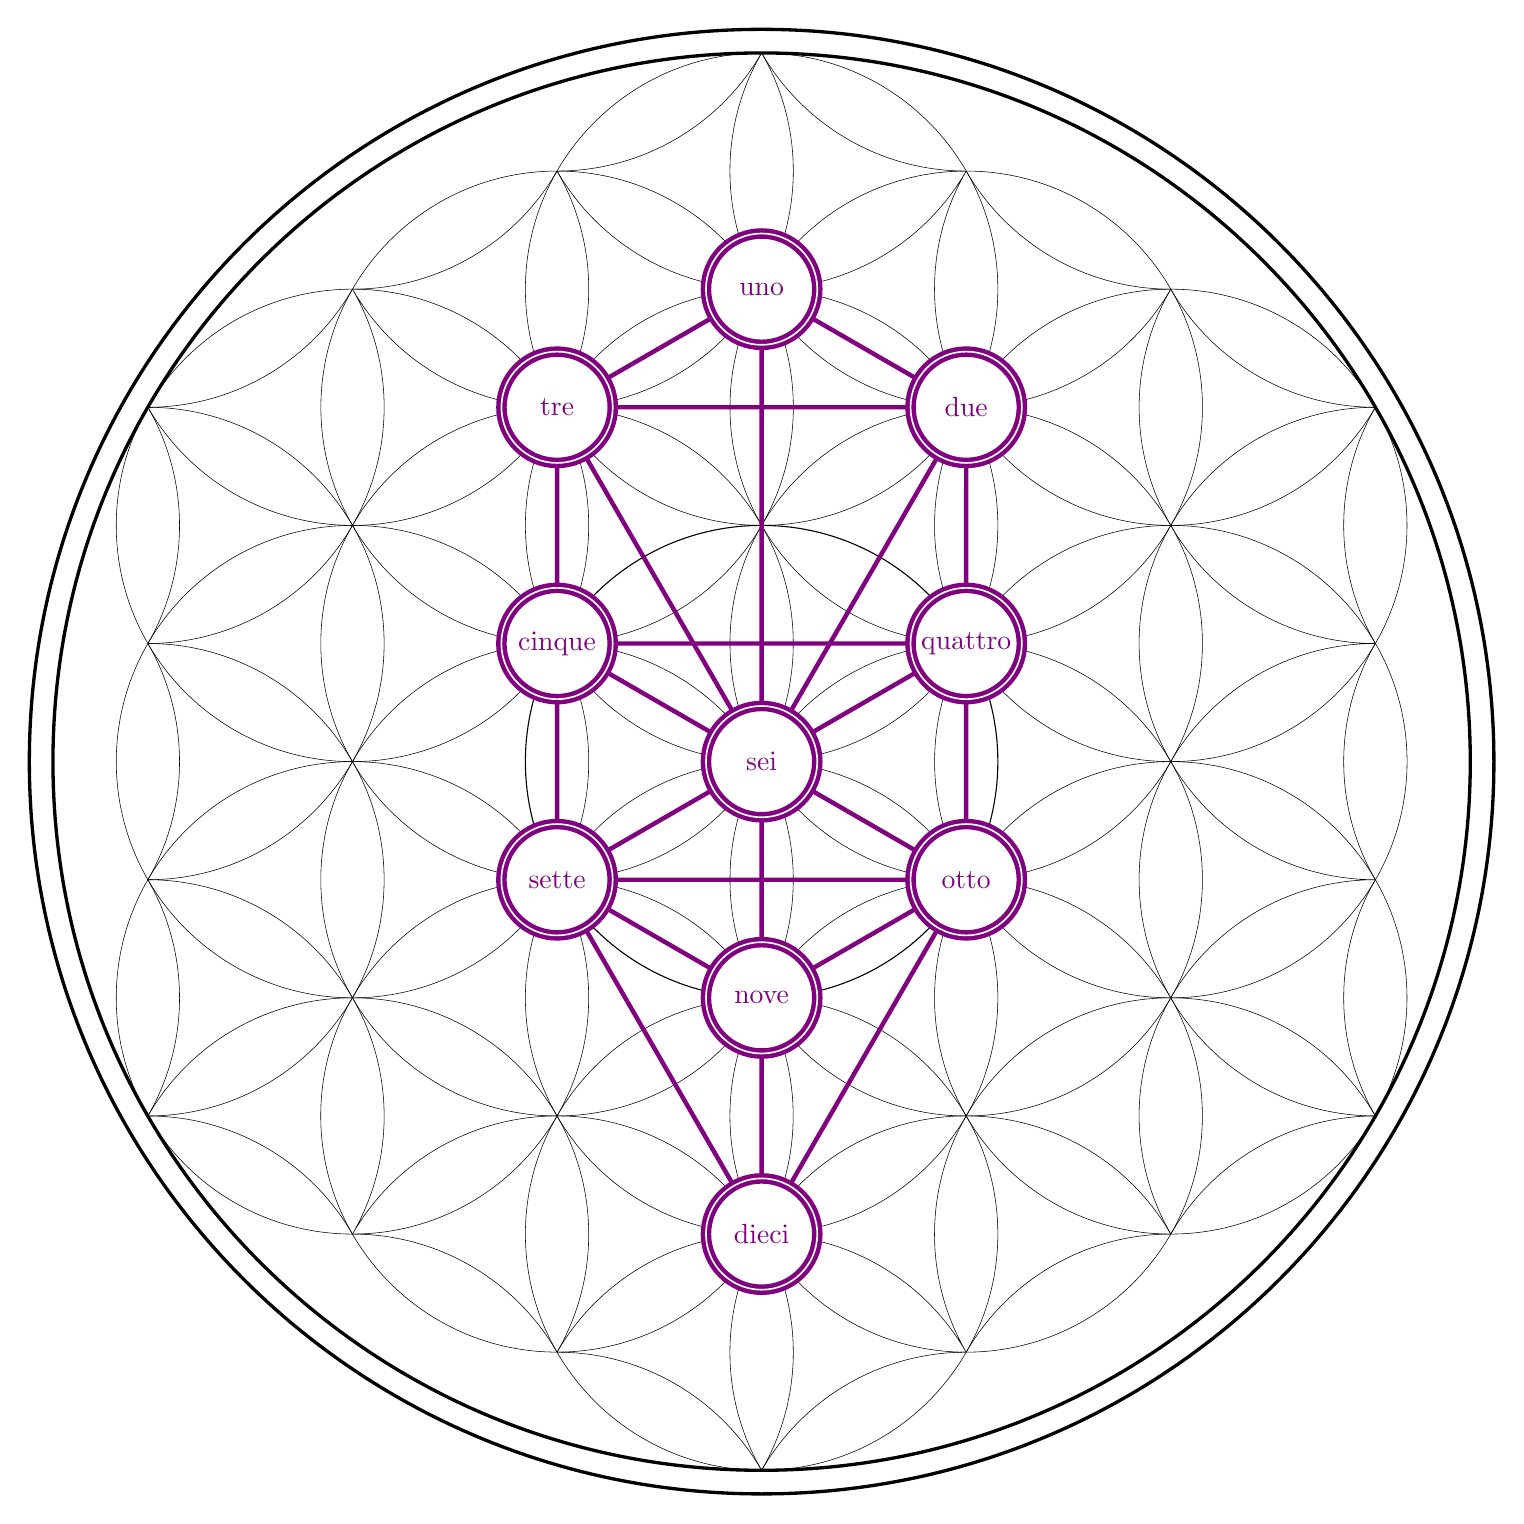
\begin{tikzpicture}
    % \draw[thick, ->] (1,0) arc (180:2:2cm);
    % \draw[thick, ->] (5,0) arc (0:-178:2cm);
    % \draw[thick] (-0.5,0) -- (6.5,0);
    \def\r{3}
    % centro
    \draw (0,0) circle (\r) coordinate (sei);
    % esagono
    \draw [very thin, name path=a30] (30:\r) circle (\r) coordinate (quattro);
    \draw [very thin, name path=a90] (90:\r) circle (\r);
    \draw [very thin, name path=a150] (150:\r) circle (\r) coordinate (cinque);
    \draw [very thin, name path=a210] (210:\r) circle (\r) coordinate (sette);
    \draw [very thin, name path=a270] (270:\r) circle (\r) coordinate (nove);
    \draw [very thin, name path=a330] (330:\r) circle (\r) coordinate (otto);
    % periferia
    %\draw (0:\r*2) circle (\r);
    \draw [very thin, name path=b30] (30:\r*2) circle (\r);
    % \draw (60:\r*2) circle (\r);
    \draw [very thin, name path=b90] (90:\r*2) circle (\r) coordinate (uno);
    % \draw (120:\r*2) circle (\r);
    \draw [very thin, name path=b150] (150:\r*2) circle (\r);
    % \draw (180:\r*2) circle (\r);
    \draw [very thin, name path=b210] (210:\r*2) circle (\r);
    % \draw (240:\r*2) circle (\r);
    \draw [very thin, name path=b270] (270:\r*2) circle (\r) coordinate (dieci);
    % \draw (300:\r*2) circle (\r);
    \draw [very thin, name path=b330] (330:\r*2) circle (\r);
    % bordo
    %\draw[red] (0,0) circle (\r*2);
    \draw[very thick] (0,0) circle (\r*3);
    \draw[very thick] (0,0) circle (\r*3.1);

    \path [name intersections={of=a30 and b30,by=b60}];
    \path [name intersections={of=a150 and b150,by=b120}];
    \path [name intersections={of=a210 and b210,by=b180}];
    \path [name intersections={of=a270 and b270,by=b240}];
    \path [name intersections={of=a330 and b270,by=b300}];
    \path [name intersections={of=a330 and b330,by=b360}];

    % \fill [] (b60) circle (2pt);
    % \fill [] (b120) circle (2pt);
    % \fill [] (b180) circle (2pt);
    % \fill [] (b240) circle (2pt);
    % \fill [] (b300) circle (2pt);
    % \fill [] (b360) circle (2pt);
    \draw [very thin, name path=b60] (b60) circle (\r);
    \draw [very thin, name path=b120] (b120) circle (\r);
    \draw [very thin, name path=b180] (b180) circle (\r);
    \draw [very thin, name path=b240] (b240) circle (\r);
    \draw [very thin, name path=b300] (b300) circle (\r);
    \draw [very thin, name path=b360] (b360) circle (\r);

    \draw [very thin] (30:\r*3) arc (90:270:\r) arc (90:210:\r);
    \draw [very thin] (30:\r*3) arc (-30:-210:\r) arc (-30:-150:\r);
    \draw [very thin] (90:\r*3) arc (30:-150:\r) arc (30:-90:\r);
    \draw [very thin] (90:\r*3) arc (-210:-30:\r);
    \draw [very thin] (150:\r*3) arc (-150:30:\r);
    \draw [very thin] (150:\r*3) arc (90:-90:\r);
    \draw [very thin] (210:\r*3) arc (150:-30:\r);
    \draw [very thin] (210:\r*3) arc (-90:90:\r);
    \draw [very thin] (270:\r*3) arc (-30:150:\r) arc (-30:90:\r);
    \draw [very thin] (270:\r*3) arc (210:30:\r);
    \draw [very thin] (330:\r*3) arc (270:90:\r) arc (270:150:\r);
    \draw [very thin] (330:\r*3) arc (30:210:\r) arc (30:150:\r);

    \draw [very thin] (90:\r*3) arc (330:270:\r) arc (330:270:\r) arc (330:270:\r)
                    arc (30:-30:\r)  arc (30:-30:\r)  arc (30:-30:\r)
                    arc (90:30:\r)   arc (90:30:\r)   arc (90:30:\r)
                    arc (150:90:\r)  arc (150:90:\r)  arc (150:90:\r)
                    arc (210:150:\r) arc (210:150:\r) arc (210:150:\r)
                    arc (270:210:\r) arc (270:210:\r) arc (270:210:\r);


    \draw[ultra thick, violet] (uno) -- (b60) -- (quattro) -- (sei) -- (cinque) -- (b120) -- (uno) -- (dieci);
    \draw[ultra thick, violet] (cinque) -- (quattro) -- (otto) -- (nove) -- (sette) -- (cinque);
    \draw[ultra thick, violet] (sette) -- (dieci) -- (otto);
    \draw[ultra thick, violet] (sette) -- (sei) -- (otto) -- (sette);
    \draw[ultra thick, violet] (b60) -- (sei) -- (b120) -- (b60);

    \tikzset{dot/.style = {draw, ultra thick, double, circle, violet, fill=white, minimum size=1.414cm,inner sep=0pt, outer sep=0pt}}

    \node [dot] (nsei) at (sei) {sei};
    \node [dot] (nquattro) at (quattro) {quattro};
    \node [dot] (ndue) at (b60) {due};
    \node [dot] (nuno) at (uno) {uno};
    \node [dot] (ntre) at (b120) {tre};
    \node [dot] (ncinque) at (150:\r) {cinque};
    \node [dot] (nsette) at (210:\r) {sette};
    \node [dot] (nnove) at (270:\r) {nove};
    \node [dot] (ndieci) at (270:\r*2) {dieci};
    \node [dot] (notto) at (330:\r) {otto};


  \end{tikzpicture}
\end{document}
